%%%%%%%%%%%%%%%%%%%%%%%%%%%%%%%%%%%%%%%%%%%%%%%%%%%%%%%%%%%%%%%%%%%%%
%% This is a (brief) model paper using the achemso class
%% The document class accepts keyval options, which should include
%% the target journal and optionally the manuscript type.
%%%%%%%%%%%%%%%%%%%%%%%%%%%%%%%%%%%%%%%%%%%%%%%%%%%%%%%%%%%%%%%%%%%%%
\documentclass[journal=jacsat,manuscript=article]{achemso}

%%%%%%%%%%%%%%%%%%%%%%%%%%%%%%%%%%%%%%%%%%%%%%%%%%%%%%%%%%%%%%%%%%%%%
%% Place any additional packages needed here.  Only include packages
%% which are essential, to avoid problems later. Do NOT use any
%% packages which require e-TeX (for example etoolbox): the e-TeX
%% extensions are not currently available on the ACS conversion
%% servers.
%%%%%%%%%%%%%%%%%%%%%%%%%%%%%%%%%%%%%%%%%%%%%%%%%%%%%%%%%%%%%%%%%%%%%
\usepackage[version=3]{mhchem} % Formula subscripts using \ce{}
\usepackage[T1]{fontenc}       % Use modern font encodings

\usepackage{color}
\usepackage{xr}
\externaldocument{suppinfo}

%%%%%%%%%%%%%%%%%%%%%%%%%%%%%%%%%%%%%%%%%%%%%%%%%%%%%%%%%%%%%%%%%%%%%
%% If issues arise when submitting your manuscript, you may want to
%% un-comment the next line.  This provides information on the
%% version of every file you have used.
%%%%%%%%%%%%%%%%%%%%%%%%%%%%%%%%%%%%%%%%%%%%%%%%%%%%%%%%%%%%%%%%%%%%%
%%\listfiles

%%%%%%%%%%%%%%%%%%%%%%%%%%%%%%%%%%%%%%%%%%%%%%%%%%%%%%%%%%%%%%%%%%%%%
%% Place any additional macros here.  Please use \newcommand* where
%% possible, and avoid layout-changing macros (which are not used
%% when typesetting).
%%%%%%%%%%%%%%%%%%%%%%%%%%%%%%%%%%%%%%%%%%%%%%%%%%%%%%%%%%%%%%%%%%%%%
\newcommand*\mycommand[1]{\texttt{\emph{#1}}}

\newcommand{\cli}{Cl$^{-}$}
\newcommand{\ki}{K$^{+}$}

%%%%%%%%%%%%%%%%%%%%%%%%%%%%%%%%%%%%%%%%%%%%%%%%%%%%%%%%%%%%%%%%%%%%%
%% Meta-data block
%% ---------------
%% Each author should be given as a separate \author command.
%%
%% Corresponding authors should have an e-mail given after the author
%% name as an \email command. Phone and fax numbers can be given
%% using \phone and \fax, respectively; this information is optional.
%%
%% The affiliation of authors is given after the authors; each
%% \affiliation command applies to all preceding authors not already
%% assigned an affiliation.
%%
%% The affiliation takes an option argument for the short name.  This
%% will typically be something like "University of Somewhere".
%%
%% The \altaffiliation macro should be used for new address, etc.
%% On the other hand, \alsoaffiliation is used on a per author basis
%% when authors are associated with multiple institutions.
%%%%%%%%%%%%%%%%%%%%%%%%%%%%%%%%%%%%%%%%%%%%%%%%%%%%%%%%%%%%%%%%%%%%%
\author{T. Miteva}
\affiliation{Sorbonne Universit\'{e}s, UPMC Univ Paris 06, UMR 7614, Laboratoire de Chimie Physique Mati\`{e}re et Rayonnement, F-75005 Paris, France}

\author{N. Kryzhevoi}
\affiliation{Theoretische Chemie, Physikalisch-Chemisches Institut, Universit\"at Heidelberg, Im Neuenheimer Feld 229, D-69120 Heidelberg, Germany}

\author{N. Sisourat}
\affiliation{Sorbonne Universit\'{e}s, UPMC Univ Paris 06, UMR 7614, Laboratoire de Chimie Physique Mati\`{e}re et Rayonnement, F-75005 Paris, France}

\author{{\color{red}Kirill ?}}
\affiliation{Theoretische Chemie, Physikalisch-Chemisches Institut, Universit\"at Heidelberg, Im Neuenheimer Feld 229, D-69120 Heidelberg, Germany}

\author{{\color{red}N. Kosugi}}
\affiliation{Institute for Molecular Science, Myodaiji, Okazaki 444-8585, Japan}

\author{Ch. Nicolas}
\affiliation{Sorbonne Universit\'{e}s, UPMC Univ Paris 06, UMR 7614, Laboratoire de Chimie Physique Mati\`{e}re et Rayonnement, F-75005 Paris, France}

\author{W. Pokapanich}
\affiliation{Sorbonne Universit\'{e}s, UPMC Univ Paris 06, UMR 7614, Laboratoire de Chimie Physique Mati\`{e}re et Rayonnement, F-75005 Paris, France}

\author{Th. Saisopa}
\affiliation{Sorbonne Universit\'{e}s, UPMC Univ Paris 06, UMR 7614, Laboratoire de Chimie Physique Mati\`{e}re et Rayonnement, F-75005 Paris, France}

\author{P. Songsiriritthigul}
\affiliation{Sorbonne Universit\'{e}s, UPMC Univ Paris 06, UMR 7614, Laboratoire de Chimie Physique Mati\`{e}re et Rayonnement, F-75005 Paris, France}

\author{Y. Rattanachai}
\affiliation{Sorbonne Universit\'{e}s, UPMC Univ Paris 06, UMR 7614, Laboratoire de Chimie Physique Mati\`{e}re et Rayonnement, F-75005 Paris, France}

\author{A. Dreuw}
\affiliation{Interdisciplinary Center for Scientific Computing, Ruprecht-Karls University, Im Neuenheimer Feld 205A, D-69120 Heidelberg, Germany}

\author{J. Wenzel}
\affiliation{Interdisciplinary Center for Scientific Computing, Ruprecht-Karls University, Im Neuenheimer Feld 205A, D-69120 Heidelberg, Germany}

\author{M. Zitnik}
\affiliation{Sorbonne Universit\'{e}s, UPMC Univ Paris 06, UMR 7614, Laboratoire de Chimie Physique Mati\`{e}re et Rayonnement, F-75005 Paris, France}

\author{R. P\"{u}ttner}
\affiliation{Sorbonne Universit\'{e}s, UPMC Univ Paris 06, UMR 7614, Laboratoire de Chimie Physique Mati\`{e}re et Rayonnement, F-75005 Paris, France}

\author{J. Palaudoux}
\affiliation{Sorbonne Universit\'{e}s, UPMC Univ Paris 06, UMR 7614, Laboratoire de Chimie Physique Mati\`{e}re et Rayonnement, F-75005 Paris, France}

\author{G. \"{O}hrwall}
\affiliation{Sorbonne Universit\'{e}s, UPMC Univ Paris 06, UMR 7614, Laboratoire de Chimie Physique Mati\`{e}re et Rayonnement, F-75005 Paris, France}

\author{J.P. Rueff}
\affiliation{Sorbonne Universit\'{e}s, UPMC Univ Paris 06, UMR 7614, Laboratoire de Chimie Physique Mati\`{e}re et Rayonnement, F-75005 Paris, France}
\affiliation{Synchrotron SOLEIL, l`Orme des Merisiers, Saint-Aubin, F-91192 Gif-sur-Yvette Cedex, France}

\author{D. C\'{e}olin}
\email{denis.ceolin@synchrotron-soleil.fr}
\affiliation{Synchrotron SOLEIL, l`Orme des Merisiers, Saint-Aubin, F-91192 Gif-sur-Yvette Cedex, France}


%%%%%%%%%%%%%%%%%%%%%%%%%%%%%%%%%%%%%%%%%%%%%%%%%%%%%%%%%%%%%%%%%%%%%
%% The document title should be given as usual. Some journals require
%% a running title from the author: this should be supplied as an
%% optional argument to \title.
%%%%%%%%%%%%%%%%%%%%%%%%%%%%%%%%%%%%%%%%%%%%%%%%%%%%%%%%%%%%%%%%%%%%%
\title[]
  {RAS + XAS study of KCl aqueous solution}

%%%%%%%%%%%%%%%%%%%%%%%%%%%%%%%%%%%%%%%%%%%%%%%%%%%%%%%%%%%%%%%%%%%%%
%% Some journals require a list of abbreviations or keywords to be
%% supplied. These should be set up here, and will be printed after
%% the title and author information, if needed.
%%%%%%%%%%%%%%%%%%%%%%%%%%%%%%%%%%%%%%%%%%%%%%%%%%%%%%%%%%%%%%%%%%%%%
\abbreviations{AES,XAS}
\keywords{Solvated metal ions, Auger spectroscopy, X-ray absorption spectroscopy}

%%%%%%%%%%%%%%%%%%%%%%%%%%%%%%%%%%%%%%%%%%%%%%%%%%%%%%%%%%%%%%%%%%%%%
%% The manuscript does not need to include \maketitle, which is
%% executed automatically.
%%%%%%%%%%%%%%%%%%%%%%%%%%%%%%%%%%%%%%%%%%%%%%%%%%%%%%%%%%%%%%%%%%%%%
\begin{document}

%%%%%%%%%%%%%%%%%%%%%%%%%%%%%%%%%%%%%%%%%%%%%%%%%%%%%%%%%%%%%%%%%%%%%
%% The "tocentry" environment can be used to create an entry for the
%% graphical table of contents. It is given here as some journals
%% require that it is printed as part of the abstract page. It will
%% be automatically moved as appropriate.
%%%%%%%%%%%%%%%%%%%%%%%%%%%%%%%%%%%%%%%%%%%%%%%%%%%%%%%%%%%%%%%%%%%%%
\begin{tocentry}

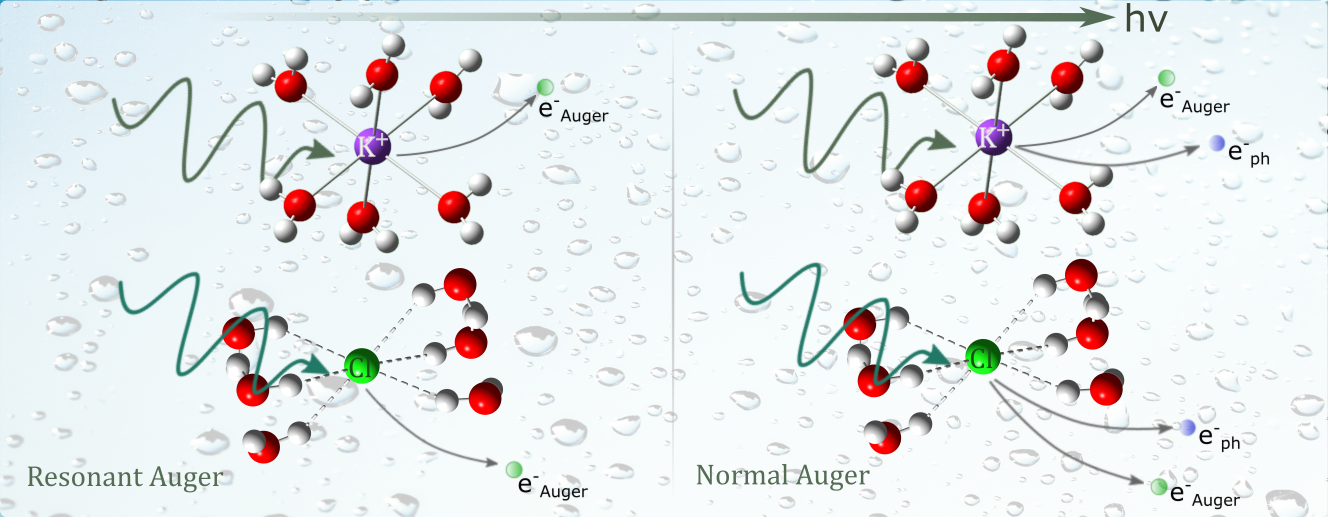
\includegraphics[scale=0.82]{figures/graphical.png}
%Some journals require a graphical entry for the Table of Contents.
%This should be laid out ``print ready'' so that the sizing of the
%text is correct.
%
%Inside the \texttt{tocentry} environment, the font used is Helvetica
%8\,pt, as required by \emph{Journal of the American Chemical
%Society}.
%
%The surrounding frame is 9\,cm by 3.5\,cm, which is the maximum
%permitted for  \emph{Journal of the American Chemical Society}
%graphical table of content entries. The box will not resize if the
%content is too big: instead it will overflow the edge of the box.
%
%This box and the associated title will always be printed on a
%separate page at the end of the document.

\end{tocentry}

%%%%%%%%%%%%%%%%%%%%%%%%%%%%%%%%%%%%%%%%%%%%%%%%%%%%%%%%%%%%%%%%%%%%%
%% The abstract environment will automatically gobble the contents
%% if an abstract is not used by the target journal.
%%%%%%%%%%%%%%%%%%%%%%%%%%%%%%%%%%%%%%%%%%%%%%%%%%%%%%%%%%%%%%%%%%%%%
\begin{abstract}
 Auger electron spectroscopy is a powerful tool to probe the electronic structure and immediate surroundings of ions in a solution. In this work we use a combination of x-ray absorption and Auger electron spectroscopies to study the electronic structure of aqueous KCl at the K-edges of \ki~and \cli. Although the two ions are isoelectronic, their Auger electron spectra as a function of the photon energy exhibit notably different features. To explain these differences, we carried out {\it ab initio} calculations of both the core excited states and the final Auger states of \ki, \cli~and their microsolvated clusters. Our calculations show that the energy order of the 3d and 4p orbitals is inverted in \ki~with respect to \cli. The reverse orbital order in the two ions not only influences their x-ray absorption spectra, but also impacts the course of the subsequent resonant Auger processes.
\end{abstract}

%%%%%%%%%%%%%%%%%%%%%%%%%%%%%%%%%%%%%%%%%%%%%%%%%%%%%%%%%%%%%%%%%%%%%
%% Start the main part of the manuscript here.
%%%%%%%%%%%%%%%%%%%%%%%%%%%%%%%%%%%%%%%%%%%%%%%%%%%%%%%%%%%%%%%%%%%%%
\section{Introduction}

XAS doesn't give information on the core-excited states

The information is contained in the combined XAS/AES spectrum

IP decreases faster than the energy of the 1st core-excited resonance

term value = IP - $E_{1st\,resonance}$ $\rightarrow$ decreases as the number of water molecules increases


The absorption of an X-ray photon by a chemical element leads to the promotion of a core-electron to empty orbitals or to the ionization continuum, which can be followed by an Auger relaxation on a femtosecond time scale or even shorter. The description of the corresponding core-excited or core-ionized states as well as of the states populated after the electronic decay provides extensive information both about the structure and the dynamics of the irradiated system (is very rich in information, both in terms of structure and dynamics of the irradiated system). These can be collected by spectroscopic methods consisting in measuring the kinetic energy of the emitted electron: Knowing the excitation energy, it is possible to determine precisely the binding energy of the ionized inner-shells, whose values are sensitive to the environment, i.e. the number and type of neighbors (electron donor or acceptor for instance). In terms of dynamics, the core-hole lifetime has been shown to be a very interesting  reference to probe ultrafast phenomena such as nuclear motion or charge transfer, both triggered by the photon absorption and occurring in particularly short time scale []. 


The Electron Spectroscopy for Chemical Analysis method (ESCA) has been extensively used in material science and atomic and molecular physics since its development in the 80’s for the reasons mentioned above. More recently, the pioneering works of M. Faubel and coworkers [] have given a new impulse since they succeeded to couple a microjet with an electron spectrometer, making it possible to track such electronic processes occurring in liquid media, especially in simple electrolyte aqueous solutions. In the last decade, a pretty large amount of new information has been collected based on this development [see e.g. references]. For instance, E.F. Aziz et al. \citep{aziz08:89} have shown that it is possible to excite the O1s orbital of OH$^-$ placed in aqueous solution, along a specific transition isolated from those of H$_2$O. The interpretation of the resonant Auger spectra coming from the relaxation of the oxygen 1s core-hole of hydroxide ion has allowed extracting information on its local environment, and on its rapid transport in water via a transition state accompanied by a mechanism of proton migration. B. Winter et al. \citep{Winter08:7130} have shown that in the case of Cl$^{-}$ ion in aqueous solution, the electronic states created by the interaction of the chlorine ion with the solvent can be populated by a resonant excitation of a Cl2p electron. These states are not visible in the  x-ray absorption spectrum, but are present in the resonant Auger spectrum. The analysis of the photon energy dependence of the energy position of the ``spectators'' states (i.e. the Cl2p electron promoted to the shared Cl/water electronic states do not participate in the relaxation) shows that they are neither completely localized nor completely delocalized but rather weakly localized around the solvated chlorine ion. The advantage of the core-orbital excitation technique is well demonstrated in this case since, in addition to the chemical selectivity, the lifetime of the core-hole gives a time base for the determination of the dynamical process: all these delocalization phenomena are almost instantaneous since they occur within the few fs of the Cl2p core-hole lifetime. The coupling chlorine - solvent is thus sufficient to allow an ultrafast charge transfer. In this article we present the results of a study focusing on the electronic structure of a KCl aqueous solution of 0.5M, excited in the vicinity of the K$^{+}$ and Cl$^{-}$ K-edges and probed by means of Auger and resonant Auger spectroscopy. After the absorption of an X-ray having an energy above the K-shell ionization thresholds, the targeted species is left with a core hole in its 1s shell and decays mostly by a KL$_{2,3}$L$_{2,3}$ Auger process, i.e. an electron from the 2p shell fills the 1s core-hole whereas a second 2p electron is ejected in the ionization continuum. For potassium and chlorine, the probability of a non-radiative decay (radiative decay) after a K-shell hole creation is about 90\% (10\%) \citep{Krause79:307}. Following this process, the electronic configuration of the final states is 2p$^{-2}$ leading to the $^1$D, $^1$S and $^3$P electronic states. In the case the 1s excited electron is not directly  ejected in the continuum but instead is promoted into an unoccupied orbital (np for a dipolar transition), then several relaxation schemes can occur. If the promoted 1s electron remains into the initially unoccupied orbital during the electronic decay, the process is called spectator Auger. The excited system 1s$^{-1}$np relaxes again mostly by involving two 2p electrons to reach the final configuration 2p$^{-2}$np. On the contrary, if at the time of the Auger decay the np electron is promoted to a n’p orbital with n’> n, then the process is called shake-up. Possibly, the np electron can fall down to an orbital n’p with n’<n, and in this case the process will be called shake-down. If the initially promoted electron is involved in the decay, the process is called participator Auger decay and the corresponding lines are shifted at higher kinetic energies compared with the spectator case. This channel will not be investigated in the present study. An additional possibility of electronic relaxation after creation of the 1s hole in potassium or chlorine ions involves neighboring water molecule. Such mechanism was for instance highlighted in a study on KCl dissolved in water and core ionized in the K$^{+}$ 2p shell \citep{Pokapanich09:7264}. The analysis of the potassium LMM Auger kinetic energy region by {\it ab initio} calculation shows that, in addition to the main lines, the extra structures located at higher kinetic energy can only be attributed to delocalized states involving both the potassium ion and water molecules. During the relaxation mechanism of the potassium 2p hole, one 3p electron of the same ion fills the core hole whereas an electron from the water valence shell is ejected in the ionization continuum. A previous study performed in the gas phase on argon (iso-electronic to Cl$^{-}$ and K$^{+}$) shows that the main relaxation channel of Ar1s excited to the first empty orbitals np ($n\geq4$), or directly ionized, leads mostly to the Ar$^+$[2p$^{-2}$]($^{1}$D$_{2}$)np or Ar$^{2+}$[2p$^{-2}$]($^{1}$D$_{2}$) final states \citep{ceolin15:022502}. The $^1$S and $^3$P states coming from the same 2p$^{-2}$ configuration were also measured but with a smaller intensity. The different mechanisms involved in the electronic decay (spectator Auger and shake processes) were clearly identified, and a formalism taking into account electronic lifetime interferences occurring in the core-excited state was used to explain the general shape of the pseudo partial cross sections 2p$^{-2}$(np) extracted from the measurements. The theory reproduces very well the experimental data and in particular it demonstrated that all the states with a 1s hole (i.e. with the excited 1s electron still bound or unbound to the system), must be coherently integrated in the model, to properly describe all the 2p$^{-2}$np and 2p$^{-2}$ pseudo cross sections. 


Thus, the main objective of this study is to collect information such as binding energy position, intensity, configuration, on the core-excited states involving a transition of the 1s orbital to either the first empty orbitals or into the ionization continuum, and to characterize the relaxation mechanisms, based on the electronic processes we highlighted for their isoelectronic counterpart in the gas phase. Potential delocalized electronic states between the solute (K$^{+}$/Cl$^{-}$) and the solvent (water) will also be probed. Our methods of investigation are the X-ray photoelectron spectroscopy and the (resonant) Auger spectroscopy in the hard X-ray range, and considering the high kinetic energy of the emitted electrons, this study is the first – to our knowledge – to clearly probe the bulk of the liquid, contrary to previous similar studies focusing on the liquid/vacuum interface. More details on the instrumental part are given in the next section.


We present {\it ab initio} calculations of the XAS spectra of microsolvated K$^{+}$(H$_2$O)$_n$ ($n = 1, 2, 4, 6$) clusters in order to interpret the experimental XAS and AES spectra. The calculations give further insight into the experimental results.

The paper is organized as follows. In the next section we present the experimental set-up and give a brief outline of the theoretical calculations. In Sec.\ \ref{sec:results} we present and discuss the results. The conclusions follow in Sec.\ \ref{sec:concl}.

\section{Methods} \label{sec:methods}
\subsection{Experimental}
% Denis, please have a look at the experimental part and see if all the references have been correctly included

For the present experiment we used the newly operational microjet setup that was specifically designed for the HAXPES station of the GALAXIES beamline, in collaboration with the Microliquids Company. Details of the beamline are given in the reference [JPR] and details on the electron spectrometer are given in the reference \citep{ceolin15:022502,ceolin13:188}. Due to the limited amount of space available if front of the analyzer lens and due to the limited number of ports available on the main vacuum chamber, the challenge was to arrange all the elements composing the microjet setup in a very compact manner. A differentially-pumped tube in which the microjet assembly is inserted, is installed in front of the spectrometer lens and can be moved independently from the main vacuum chamber by means of a three axes motorized manipulator. Two holes of 2 mm diameter allow the photons to go in and out of the tube, and a third one, on which is mounted a skimmer having a 500$\mu$m diameter hole, allows the electrons created at the interaction point to go in the direction of the spectrometer lens. To ensure a proper vacuum in the differentially pumped tube, a 5-way cross is connected to it and holds a 1200 l/s turbo pump, a liquid nitrogen trap, a vacuum gage and the liquid/electrical feedthroughs. A rail, fixed at the bottom of the tube, is used to slides precisely an insert on which the different elements necessary for the injection, control, collection and visualization of the liquid are mounted.


The head of this insert is mostly composed by: a glass capillary fixed by a dedicated peek-piece, a catcher in CuBe with a 300$\mu$m hole, a piezo motors stage allowing a precise control of these last two parts, and a camera. The catcher is placed at a distance of about 5mm from the capillary and is permanently pumped in order to extract the liquid from the vacuum chamber. For the present experiment, a 0.5M KCl aqueous solution is injected in a capillary having a 30$\mu$m diameter, by a HPLC pump with a constant flux of 1.6 ml/min. The catcher temperature is controlled so that the liquid does not freeze before its extraction. Considering that the photon propagation axis, the spectrometer lens axis and the liquid microjet form an orthogonal trihedron, the piezo motorization allows moving the liquid microjet along the photon propagation and the lens axes during the experiment if necessary. The catcher can be moved by the piezo motors along the photon propagation axis only. A simple camera is used to control the liquid jet positioning as compared with the catcher hole. The alignment of the full head (particularly capillary plus catcher) as compared with the X-ray beam is performed by moving the whole system using the 3-axes motorized manipulator. The alignment of the setup is performed by measuring the O1s XPS peak intensity of a simple salt aqueous solution, and by optimizing the liquid phase vs gas phase ratio. The pressure in the main chamber was kept below the 10$^{-5}$ mbar range whereas it was kept at about 10$^{-4}$ mbar in the differentially pumped tube when the HPLC pump was ON. Our equipment is an updated version of the equipment used in the references [3-5]. The aqueous potassium chloride solution was prepared by mixing >99\% KCl salt with deionized water. Filtering and degazing procedures were systematically performed before injecting the solution into the microjet by the HPLC pump.


\subsection{{\bf{\it Ab initio}} calculations}

The X-ray absorption spectra of the microsolvated clusters of potassium and chlorine were computed at the ground state equilibrium geometries of K$^+$(H$_2$O)$_m$ and \cli(H$_2$O)$_m$, where m = 1, 2, 4, 6. All structures were optimized at the MP2 level of theory using the 6-311++G(2d,2p) basis set \citep{Krishnan80:650,Blaudeau97:5016}. A frequency analysis was carried out in order to confirm that the obtained geometries are minima on the respective potential energy surfaces. The geometry optimization and frequency analysis were performed with the Gaussian 09 package \citep{g09}. In the case of K$^{+}$(H$_2$O)$_6$ the ground state geometry was obtained by constrained geometry optimization starting with the equilibrium geometry \citep{lee99:3995} belonging to the D$_3$ point group and increasing the angle $\theta$ between the K-O bond and the $C_3$ axis to 55$^{\circ}$. This angle was chosen to be around the maximum in the O-K-O angular distribution obtained from quantum mechanics / molecular mechanics dynamical simulations in Ref.\ \citep{ma14:1006}. {\color{red} the maximum is at 70$^{\circ}$, in our calculation the angle is 90$^{\circ}$} The ground state equilibrium structures are presented in Figs.\ \ref{fg:knw_xas} and \ref{fg:clnw_xas}. In the case of potassium, they belong to the C$_{2\text{v}}$ (K$^{+}$(H$_2$O)), D$_{2\text{d}}$ (K$^{+}$(H$_2$O)$_2$), S$_4$ (K$^{+}$(H$_2$O)$_4$), and D$_3$ (K$^{+}$(H$_2$O)$_6$) point groups \citep{rao08:12944}. The optimized K-O distances are between 2.638 -- 2.842~\AA, which is in good agreement with other theoretical and experimental works \citep{Ohtaki93:1157,soper06:180,ma14:1006}. In the case of chlorine, the ground state equilibrium 1-, 2- and 6-coordinated structures belong to the C$_{1}$ point group, whereas the 4-coordinated structure belongs to the C$_4$ point group \citep{gora00:7}. The optimized Cl-O distances are between 3.093 -- {\color{red}3.305}~\AA, which is in good agreement with other theoretical and experimental works \citep{ge13:13169,gora00:7,Ohtaki93:1157,soper06:180,ma14:1006}. The 6-coordinated clusters can be considered as representatives of the complete first solvation shell of the two ions \citep{Ohtaki93:1157,soper06:180,ma14:1006}.


The energies and transition moments of the core excited states of the microsolvated clusters were computed with the algebraic diagrammatic construction method for the polarization propagator \citep{sch82:2395} within the core-valence separation approximation \citep{bar85:867,ced80:206,ced81:1038} (CVS-ADC(2)x) as implemented in the Q-Chem package \citep{Wenzel14:1900,Wenzel14:4583,Wormit14:774,QChem2015}. In the case of \cli, the 6-311++G(3df,3pd) basis set \citep{Krishnan80:650,McLean80:5639} (excluding the f functions) was used on all atoms, whereas in the case of \ki, we used the 6-311+G(2d,p) basis set \citep{Krishnan80:650,Blaudeau97:5016} on all atoms, and an additional set of 2s, 2p and 2d diffuse functions was added on K. In our calculations, the core space comprises the 1s orbital of K$^{+}$ or \cli, whereas the remaining occupied orbitals are included in the valence space. For the calculations of the XAS spectra we used the D$_2$ point group in the case of K$^{+}$(H$_2$O)$_2$, the C$_2$ point group in the case of K$^{+}$(H$_2$O)$_4$, K$^{+}$(H$_2$O)$_6$ and \cli(H$_2$O)$_4$. To account for the experimental resolution and for the lifetime broadening due to the Auger decay of the core excited states, we convolved the theoretical spectra with a {\color{red} (Denis, exp. resolution? ) Voigt profile with a Gaussian of FWHM XX\,eV} and a Lorentzian of FWHM 0.74\,eV and 0.62\,eV in the case of \ki~and \cli, respectively \citep{Krause79:329}. We analyzed the core excited states by expanding the singly occupied natural orbitals (SONOs) $\psi_{i}$ of the microsolvated clusters in the basis of SONOs of the bare K$^{+}$ or \cli~ion $\chi_{nl}$
%
\begin{equation}\label{eq:sono_proj}
\psi_{i} = \sum_{nl} a^{i}_{nl} \chi_{nl}
\end{equation}
%
where $n$ and $l$ stand for the principal and orbital quantum numbers as described in Ref.\ \citep{miteva16:16671}. The expansion coefficients $a^{i}_{nl}$ show the degree of delocalization of the excited electron and the mixing of the core excited states in the crystal field created by the surrounding water molecules (see Figs.\ \ref{fg:knw_xas} and \ref{fg:clnw_xas}).


The final states following KLL resonant Auger decay of K$^{+}$ and \cli~were computed at the Configuration Interaction Singles (CIS) level using the Graphical Unitary Group Approach (GUGA) as implemented in the GAMESS-US package \citep{GUGA_PhysScr_21,GUGA_JCP_70,GUS}. We used the 6-311++G(2d,2p) basis set \citep{Blaudeau97:5016} augmented with 2s, 2p, 2d diffuse functions on \ki, and the cc-pVTZ basis set augmented with 6s, 6p, 6d diffuse KBJ functions \citep{Kaufmann89:2223} on \cli. The active space comprises the 2s and 2p orbitals of K/Cl with occupancy fixed to 6 and all virtual orbitals with occupancy fixed to 1. The remaining doubly occupied orbitals were frozen in the calculation. \citep{mosnier16:061401}

\section{Results}\label{sec:results}

% Question to Denis: how exactly do you extract the IP from the XPS spectrum?
%{\color{blue}
%THESE RESULTS ARE ALREADY reported in the other paper, so we don't need them here, do we?
%
%The ionization potentials (IP) of Cl$^{-}$1s and K$^{+}$1s were measured by XPS at $h\nu = 5$\,keV, far enough from the threshold to minimize PCI effects, and calibrated on the O1s (liquid) binding energy taken at 538.1\,eV \citep{winter06:1176}. We found the value of 2825.4\,eV for the ionization potential of Cl$^{-}$ 1s (Fig.\ \ref{fg:2dmap_cl}) and 3611.9\,eV for K$^{+}$ 1s (Fig.\ \ref{fg:2dmap_k}). The full width half-maximum of these main lines was extracted and their Lorentzian contribution was measured at 0.72\,eV for K$^{+}$1s(aq) and 0.62\,eV for Cl$^{-}$1s(aq). This result agrees well with the corresponding theoretical values of 0.74\,eV and 0.64\,eV for bare potassium and chloride taken from Ref.\ \citep{Krause79:329}. In the X-ray energy region of the ionization potential of aqueous Cl$^{-}$, the photon bandwidth provided by the double crystal monochromator is about {\color{red}0.4\,eV}, whereas in the region of the ionization potential of aqueous K$^{+}$, the photon bandwidth is about {\color{red}0.5\,eV}.}


In this section we discuss the experimental results presented as 2D maps showing the dependence of the kinetic energy of the Auger electrons on the photon energy scanned across the K-edges of the aqueous potassium, 3611.9\,eV (Fig.\ \ref{fg:2dmap_k}), and chloride ions, 2825.4\,eV (Fig.\ \ref{fg:2dmap_cl}) \citep{ceolin17}. First, we present the normal Auger part of the spectra, then we discuss the resonant Auger features. The range of electron kinetic energies of the corresponding relaxation channels is larger than 2\,keV, which corresponds to inelastic mean free paths of about 50~\AA~or more in liquid water \citep{emfiet09:45}. The energies thus allow us to probe the bulk of the sample and, moreover, they ensure that the electrons escape the liquid with a sufficient count rate.




\begin{figure}%[h!]
\centering
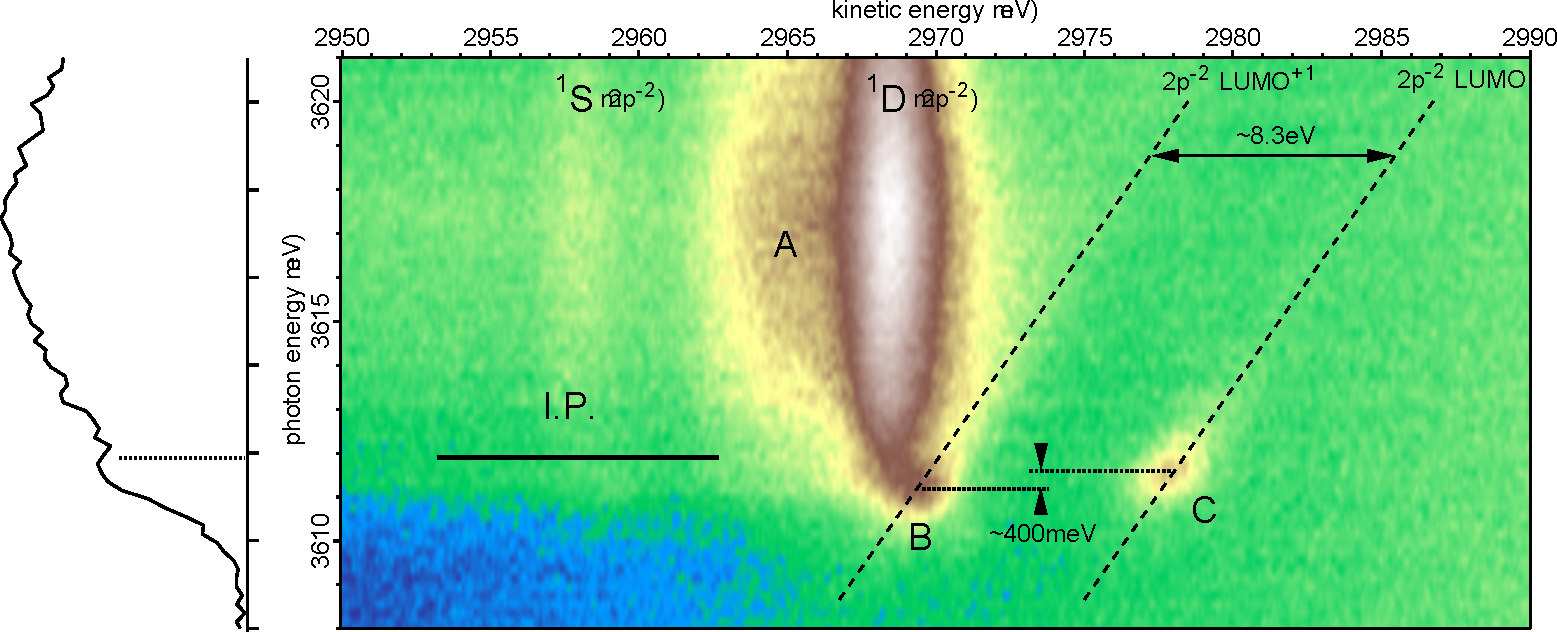
\includegraphics[scale=0.55]{figures/2Dmap_K1s_XAS.pdf}
\caption{2D map showing the kinetic energy of the electrons emitted in $K L_{2,3}L_{2,3}$ Auger decay vs the photon energy in the vicinity of the K-edge of aqueous K$^{+}$. The black curve on the left represents the experimental partial electron yield spectrum of K$^{+}$ obtained after integrating over the kinetic energies of the Auger electrons.\\
{\color{red}\bf @Denis, can you please add the letters B and C on the 2D map, and also make the 2D maps of \ki~and \cli~the same size and use the same font size?}}
\label{fg:2dmap_k}
\end{figure}


\begin{figure}%[h]
\centering
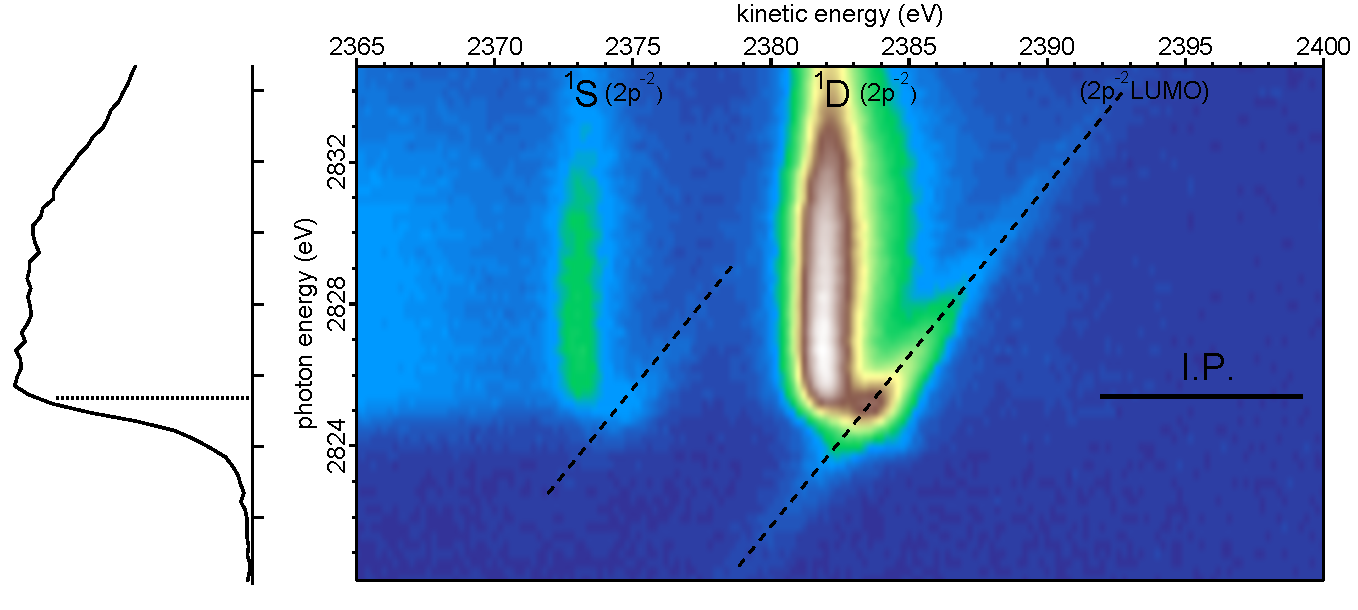
\includegraphics[scale=0.65]{figures/2Dmap_Cl1s_XAS.pdf}
\caption{2D map showing the kinetic energy of the electrons emitted in $K L_{2,3}L_{2,3}$ Auger decay vs the photon energy in the vicinity of the K-edge of aqueous Cl$^{-}$. The black curve on the left represents the experimental partial electron yield spectrum of Cl$^{-}$ obtained after integrating over the kinetic energies of the Auger electrons.}
\label{fg:2dmap_cl}
\end{figure}


\subsection{Normal Auger decay}\label{ssec:na}

Let us first consider the vertical lines at photon energies $h\nu = 3617$\,eV {\color{red}(spectrometer resolution)} on Fig.\ \ref{fg:2dmap_k} and $h\nu = 2830$\,eV {\color{red}(spectrometer resolution)} on Fig.\ \ref{fg:2dmap_cl}, respectively. They originate from KL$_{2,3}$L$_{2,3}$ Auger decay following the core ionization of K$^+$ and Cl$^-$, which leads to the population of $^3$P, $^1$D, and $^1$S $2p^{-2}$ final states
%
\begin{align*}
h\nu + \text{K}_\text{aq}^{+} \rightarrow \text{K}_\text{aq}^{++}(1s^{-1}) + e^{-}_{\text{ph}}
			 \rightarrow \text{K}_\text{aq}^{3+} (2p^{-2}\ \ ^3\text{P},\ ^1\text{D},\ ^1\text{S}) + e^{-}_{\text{ph}} + e^{-}_{\text{Auger}} \\
h\nu + \text{Cl}_\text{aq}^{-} \rightarrow \text{Cl}_\text{aq}^{0}(1s^{-1}) + e^{-}_{\text{ph}}
			 \rightarrow \text{Cl}_\text{aq}^{+} (2p^{-2}\ \ ^3\text{P},\ ^1\text{D},\ ^1\text{S}) + e^{-}_{\text{ph}} + e^{-}_{\text{Auger}} 
\end{align*}
%
In the case of Cl$^{-}_{\text{aq}}$, the lines corresponding to the Cl$^{+}$ (2p$^{-2}$) $^1$S, $^1$D and $^3$P states are located at 2373.2\,eV, 2382.1\,eV and $\sim$2390\,eV kinetic energy. The position of the $^{3}$P line is determined approximately as the line is obscured by the dispersive feature with a maximum at 2825.2\,eV photon energy and 2383.5\,eV kinetic energy (see Fig.\ \ref{fg:2dmap_cl}). For K$^{+}_{\text{aq}}$ the maxima of the $^1$S and $^1$D KL$_{2,3}$L$_{2,3}$ Auger lines are located at 2958\,eV and 2968.4\,eV, respectively (see Fig.\ \ref{fg:2dmap_k}). The intensity of the $^3$P line is too weak and it cannot be clearly distinguished as it is obscured by the high-kinetic energy tail of the $^1$D line and by one of the dispersive lines with a maximum at 2969.5\,eV.


The KL$_{2,3}$L$_{2,3}$ Auger lines are not supposed to disperse with the photon energy except close to threshold due to the interaction between the photoelectron and Auger electron, i.e.\ the so-called post-collision interaction (PCI). As a result of this interaction, first, the peaks in the Auger spectrum become asymmetric with a shoulder at high kinetic energies, and second, they are shifted to higher kinetic energies close to threshold \citep{russek86:911,guillemin15:012503}. Consequently, one can attribute the high kinetic energy shoulder of the $^1$D and $^1$S peaks on Figs.\ \ref{fg:2dmap_k} and \ref{fg:2dmap_cl} as resulting from PCI effect. In order to minimize this effect we recorded the KLL Auger spectrum of both Cl$^{-}_{\text{aq}}$ and K$^{+}_{\text{aq}}$ at higher photon energies, $h\nu = 5$\,keV. The maxima of the $^3$P, $^1$D and $^1$S states were found at 2389\,eV, 2381.1\,eV and 2372.3\,eV for Cl$^{-}_{\text{aq}}$, and 2976.3\,eV, 2967.4\,eV and 2957\,eV kinetic energy for K$^{+}_{\text{aq}}$, respectively. The lines observed at a photon energy far from threshold and close to it appear to be shifted by $\sim$1\,eV. The magnitude of the shift is the same for both ions, thus, we can conclude that it does not depend on the initial charge of the ion. The observed PCI shift of 1\,eV is larger than in the case of the isoelectronic Ar, where its value is $\sim$0.5\,eV at a photon energy of 10 \,eV above threshold \citep{guillemin15:012503}. The shift in the energies of the photo- and Auger electrons is proportional to the change in the ionic field during the Auger process. In a solution, both the single and double ionization potentials change due to the stabilization of the ionic species through ion-dipole interaction with the polarizable medium. For example, in \ki, the ionization potential of the bare ion was experimentally determined to be 3619.4\,eV \citep{hertlein06:062715}, whereas in an aqueous solution, its value drops to 3611.9\,eV, i.e.\ by about 7\,eV. The magnitude of this effect increases with the ionic charge, consequently, there will be an even greater difference for the double ionization potential. Thus, one can expect a larger change in the ionic field in an aqueous solution compared to that in a van der Waals cluster, which can, therefore, account for the large PCI shift of the Auger lines in a solution.


The normal Auger $^1$D main line of K$^{+}$ differs from that of Cl$^{-}$ by the presence of a large shoulder on the low kinetic energy side at about 2965\,eV kinetic energy. This shoulder is a result of a charge transfer process to the solvent molecules which will be the subject of a separate article \citep{ceolin17}.


\subsection{Resonant Auger decay} \label{ssec:ra}
Next, we discuss the dispersive features in the spectra of aqueous \ki~and \cli~originating from the resonant Auger decay of the core excited states below threshold. In order to get a better understanding of these features, we will first consider the Auger spectrum of the isoelectronic Ar presented in Refs.\ \citep{ceolin15:022502,guillemin15:012503}. 


First, from the 2D map of Ar one can extract information about the nature of the core excited states below threshold. The pre-edge structure in the XAS spectrum of Ar consists of the 1s$\,\rightarrow\,$4p and 1s$\,\rightarrow\,$5p excitations. Higher core excited states cannot be identified in the XAS spectrum due to their lifetime broadening and proximity to the ionization threshold. The same excitations were observed in the XAS spectrum of bare \ki~ions \citep{hertlein06:062715}. Again, the identification of 1s$\,\rightarrow\,$np states with n$\,>\,$5 was not possible in the case of \ki.


Second, the 2D map of Ar carries information about the states populated in the resonant Auger processes following core excitation. In the case of Ar, the Ar 1s$\,\rightarrow\,$4p and 1s$\,\rightarrow\,$5p core excited states undergo both pure spectator and shake-up resonant Auger decay leading to the population of Ar$^{2+}$(2p$^{-2}$np) (n$ = 4 - 6$) final states. As a result, apart from the main Ar$^{2+}(2p^{-2})$ $^1$D and $^1$S lines which result from normal Auger decay, additional dispersive features are observed. For example, the 1s$\,\rightarrow\,$4p core excited state undergoes both pure spectator and shake-up resonant Auger decay. The former results in an island shifted with respect to the main $^1$D line by $\sim$4-5\,eV kinetic energy, whereas the fingerprint of the shake-up process is a feature appearing at the same kinetic energy as the  main $^1$D line. Moreover, the intensities of the observed shake-up features are lower compared to those of the pure spectator Auger decay. In aqueous solutions, one can expect the 2D map to be fairly different as both the initial core excited states and the final Auger states will be influenced by the presence of the solvent.


The dispersive features on the 2D map of \cli~(Fig.\ \ref{fg:2dmap_cl}) are designated by dashed lines. The maxima of these features are located at 2825.2\,eV photon energy, i.e.\ only 0.2\,eV below the $1s$ ionization potential of Cl$^{-}_{\text{aq}}$. Due to the natural lifetime broadening of 0.62\,eV \citep{Krause79:329} of both the core excited and core ionized states of Cl, no pre-edge structure is observed in the XAS spectrum presented to the left on Fig.\ \ref{fg:2dmap_cl}. The excitation energy of 2825.2\,eV agrees very well with the position of the Cl$^{-}$ 1s$\,\rightarrow\,$4p excitation determined by Cl K-edge XAS experiments in MgCl$_2$.6H$_2$O and of SrCl$_2$/SrCl$_2$.6H$_2$O \citep{sugiura82:681} and MCl$_{4}^{-}$ compounds \citep{shadle95:2259}. Contrary to the case of Ar, with which Cl$^{-}$ is isoelectronic, a separate shake-up feature is not observed on the 2D map of \cli$_{\text{aq}}$.


%{\color{red} {\bf @Denis, can you please have a look at this paragraph from the original version of the paper you sent me, I didn't quite understand it.} However, for atomic chloride, the description of the excited states in terms of Rydberg series is possible because the promoted electron sees an ionic core of a +1 charge. In the case of chlorine, the situation is different since the charge seen by the 1s promoted electron is null and thus using a Rydberg series description is not appropriate. More generally, it is known that isolated halide ions have no bound excited states (Berry, R. S.; Reimann, C. W.; Spokes, G. N. J. Chem. Phys. (1962), 37, 2278, Wen-Shyan Sheu and Peter J. Rossky, J. Phys. Chem. (1996), 100, 1295). However, when surrounded by water molecules, delocalized states as CTTS states have been highlighted by various MD simulations (Staib, A.; Borgis, D., J. Chem. Phys. 104, (1996), 9027 and J. Chem. Phys. 103, (1995) 2642) and experimental methods, including resonant Auger spectroscopy performed in the vicinity of the Cl-2p ionization threshold, as demonstrated by Winter et al. (JACS, 130 (2008) 7130). In the present case, we excite a s-type symmetry orbital so we expect to populate mostly p-type orbital(s). Staib, A.; Borgis, D., (J. Chem. Phys. 104, (1996), 9027 and J. Chem. Phys. 103, (1995) 2642) have calculated density of states for Cl-(aq) and highlighted a dense manifold of p-symmetry states followed by s/d symmetry states in an energy region just below the electron photo detachment threshold value, i.e., from about -1 eV to 0 eV. In our case, the 1s-1-first unoccupied state maximum is at about 0.2eV below threshold, but the corresponding core-excited state has a natural broadening of about 0.6 eV FWHM, meaning thus that the core-excited states overlap (SORRY, here again I need to add arguments).}


The 2D map corresponding to the relaxation of solvated potassium ion excited in the vicinity of its K-edge is presented on Fig.\ \ref{fg:2dmap_k}. Two dispersive feature are observed. They have maxima at $h\nu = $3611.2 \,eV and 2969.2 \,eV kinetic energy (feature B), and $h\nu = $3611.6\,eV and 2978.1\,eV kinetic energy (feature C), respectively. Dispersive feature C appears as an island, separated by approximately 400\,meV photon energy and 8.3\,eV kinetic energy from B, which on its turn is close to the $^1$D main line. Unlike in the case Cl$^{-}$ the dispersive feature close to the $^1$S main line is not observed in K$^{+}$ due to presence of a strong {\color{red}background (@DENIS?)}. These two core-excited states are close in energy to the energy of the 1s$\,\rightarrow\,$4p excitation in bare \ki, 3610.7\,eV \citep{hertlein06:062715}. Again due to the lifetime broadening, the core excited states cannot be distinguished in the XAS spectrum to the left on Fig.\ \ref{fg:2dmap_k}.

\section{Discussion}\label{sec:disc}

\begin{figure}
\centering
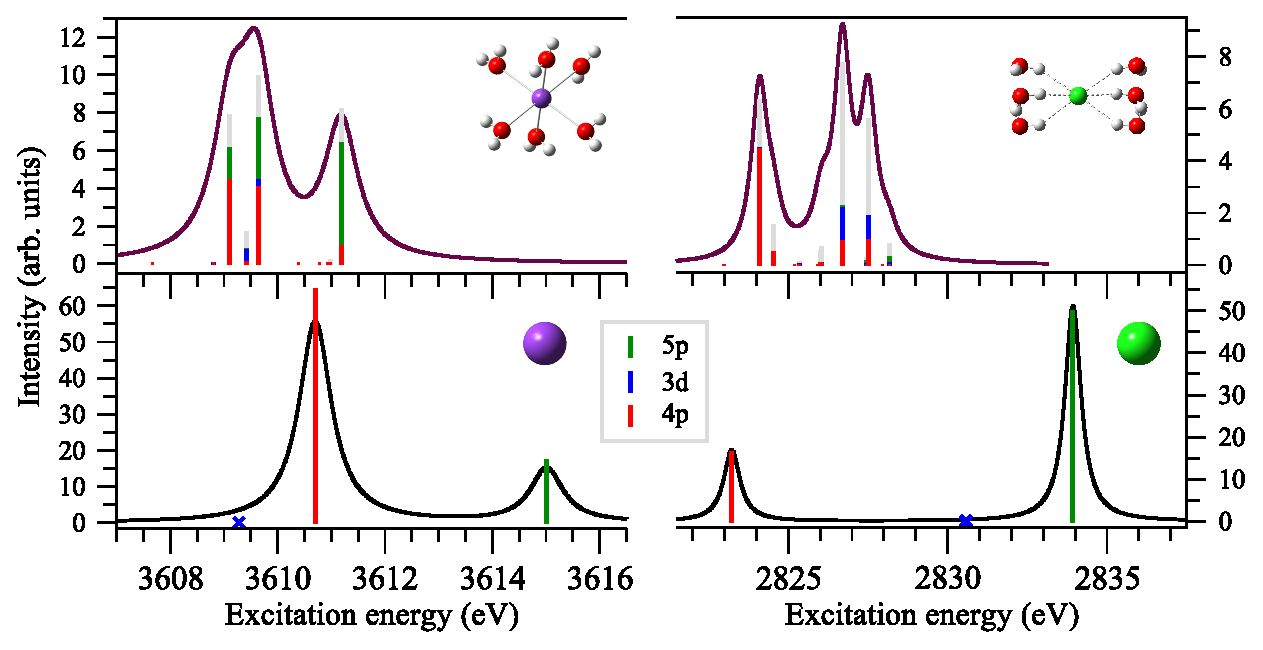
\includegraphics[scale=0.6]{figures/xas_spectra.eps}
\caption{
XAS spectra of the lowest K-shell transitions in the bare K$^{+}$ (lower left panel) and Cl$^{-}$ (lower right panel) ions and their 6-coordinated clusters (upper left panel, \ki(H$_2$O)$_6$, and upper right panel, \cli(H$_2$O)$_6$). The theoretical stick spectra were convolved with a Lorentzian profile of FWHM 0.74\,eV for \ki~and 0.62\,eV for \cli~in order to account for the lifetime broadening. The stick spectrum corresponds to the projections $|a_{nl}^{i}|^2$ of the SONOs corresponding to the core excited states of the 6-coordinated clusters on the basis of SONOs corresponding to the 1s$\,\rightarrow\,$3d, 1s$\,\rightarrow\,$4p, and 1s$\,\rightarrow\,$5p states in the bare K$^+$ and \cli~ions (Eq.\ \ref{eq:sono_proj}). The theoretical XAS spectra of \ki~were shifted to higher photon energies by 6.7\,eV, which corresponds to the difference between the computed and experimental core excitation energies of the 1s $\rightarrow$ 4p excitation in the bare ion taken from Ref.\ \citep{hertlein06:062715}.}
\label{fg:xas_kcl}
\end{figure}


In order to understand the resonant Auger features in the experimental AES spectra we computed the X-ray absorption spectra of both \ki~and \cli~and their microsolvated clusters with 1, 2, 4 and 6 water molecules, as well as the final Auger states of the bare ions.


The theoretical XAS spectra are presented in Figs.\ \ref{fg:xas_kcl} and \ref{fg:xas_kcl}. For both \ki~and \cli~(lowermost panels), the first observed peak in the XAS spectrum corresponds to the 1s$\,\rightarrow\,$4p state. It is noteworthy that the positions of the 1s$\,\rightarrow\,$4p and 1s$\,\rightarrow\,$3d states are inverted in \ki~and \cli. In the case of Cl$^{-}$ the 1s$\,\rightarrow\,$4p excitation has lower energy and the 1s$\,\rightarrow\,$3d excitation is close to the 1s$\,\rightarrow\,$5p state. On the contrary, in K$^{+}$ the 1s$\,\rightarrow\,$3d excitation has lower energy and lies below the 1s$\,\rightarrow\,$4p state. It is noteworthy that the intensity of the 1s$\,\rightarrow\,$4p state is lower than that of the 1s$\,\rightarrow\,$5p state in \cli. An explanation of this phenomenon can be found in the Supporting Information.


%1.4 Solvated clusters:

In what follows, we will focus on the fate of the lowest-lying peak in the XAS spectra of \ki~and \cli, originating from the excitation of a 1s electron to the 4p unoccupied orbital (Figs.\ \ref{fg:xas_kcl} and \ref{fg:xas_kcl}). In the case of \ki~the position of the peak drops from 3610.7\,eV in the bare ion \citep{hertlein06:062715} to 3608.7\,eV in the 4-coordinated cluster, whereas in the case of \cli~the solvent molecules have little influence on the position of the first peak (it varies between 2823.3\,eV for the ion and 2824.2\,eV for the 6-coordinated cluster). Since the peak is broadened due to the finite lifetime and the splitting of the core excited states in the ligand field of the solvent, and because the 1s ionization potential of \ki~drops by $\sim$7\,eV in a solution \citep{ceolin17} compared to the bare ion \citep{hertlein06:062715}, which is more than the difference between the 1s$\,\rightarrow\,$4p and 1s$\,\rightarrow\,$5p states, we expect that these states are the only states populated below the ionization threshold.


Let us first consider how the 1s$\,\rightarrow\,$4p core excitation of \ki~is influenced by the presence of the solvent (see Fig.\ \ref{fg:xas_kcl}). In the singly- and doubly-coordinated clusters, the 1s$\,\rightarrow\,$4p excitation splits into groups of states, which results in the formation of a low-intensity shoulder on the high photon energy side of the main peak in the theoretical XAS spectra. The situation is substantially different for the 4-coordinated clusters, where the first peak in the XAS spectrum is produced by states with a small contribution from the dipole allowed 1s$\,\rightarrow\,$4p state and a large contribution $\sim$40\% from the dark 1s$\,\rightarrow\,$3d states. The latter states acquire intensity due to mixing with the 4p-states in the ligand field created by the solvent. A similar effect was observed in the microsolvated clusters of Na$^{+}$ and Mg$^{2+}$ \citep{miteva16:16671}. Finally, in the 6-coordinated cluster, which represents the complete first solvation shell around \ki, the lowest peak in the spectrum contains the 1s$\,\rightarrow\,$4p states split by approximately 0.5\,eV, and a low intensity state in between, which has a predominantly 1s$\,\rightarrow\,$3d character, and which also acquires intensity due to mixing with the bright 4p- and 5p-core excited states.


In the case of \cli, the water molecules tend to gather on one side of the \cli~ion and form H-bonds with it \citep{ge13:13169}. The resulting structures are of lower symmetry compared to the respective microsolvated clusters of \ki, which influences the splitting of the states of the bare ion upon the addition of solvent molecules (Fig.\ \ref{fg:xas_kcl}). This effect is most pronounced for the higher lying 1s$\,\rightarrow\,$5p states and it does not substantially. The lowest lying 1s$\,\rightarrow\,$4p excitation in \cli~can still be identified in the microsolvated clusters. Moreover, this state does not interact strongly with the 1s$\,\rightarrow\,$3d state because as earlier discussed, they do not lie close in energy in the bare ion.


\begin{figure}[h!]
\centering
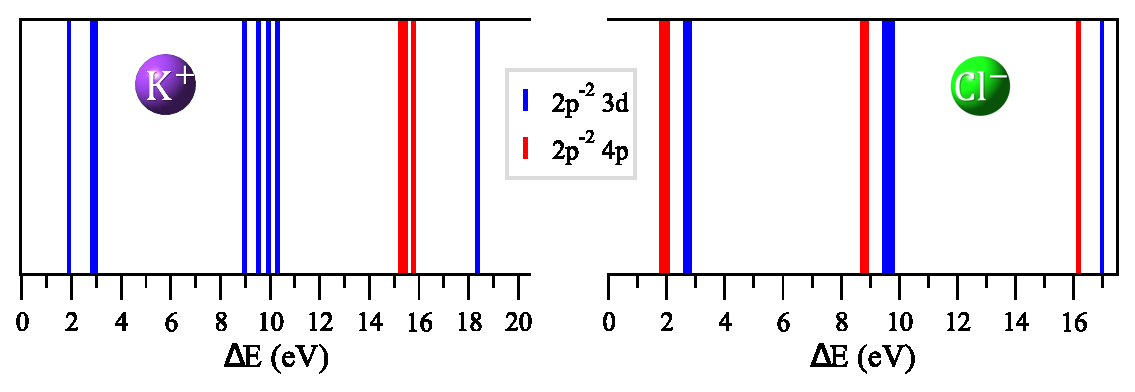
\includegraphics[scale=0.6]{figures/kcl_2p-2nl.eps}
\caption{Final 2p$^{-2}$($^3$P, $^1$D) 3d, 4s, 4p doublet Auger states of K$^{+}$ (left) and Cl$^{-}$ (right) computed at the CIS level (see Sec.\ \ref{sec:methods} for details). The states are shifted with respect to the lowest quartet state with electron configuration 2p$^{-2}$($^3$P) 4s.}
\label{fg:kcl_2p4nl}
\end{figure}


Solely from the XAS spectra, one cannot extract information about the course of the subsequent Auger process. As can be seen on the 2D maps of \ki~and \cli, the resonant Auger process is the decay pathway of the lowest lying core excited states. In what follows, we attempt to explain the dispersive features in the experimental spectra of \ki~and \cli,~and understand the interrelation between the electronic structure of the core excited species and their Auger electron spectra. To this end we computed the lowest K$^{2+}$(2p$^{-2}$nl) and Cl$^{0}$(2p$^{-2}$nl) states corresponding to the lowest final spectator resonant Auger states (Fig.\ \ref{fg:kcl_2p4nl}). Out of all final states we discuss only the doublets assuming that the quartet states are populated with a very low probability (REFS). Already at the level of the bare ion one can see that the 2p$^{-2}$nl states of \ki~and \cli~are substantially different. They reflect the fact that the 3d unoccupied orbitals of \ki~are lower than the 4p orbitals, which is the opposite of what is observed in \cli.


The lowest doublet states of \ki~are the 2p$^{-2}$3d states, they form two groups of states around 2\,eV and 10\,eV above the lowest quartet state. The lowest 2p$^{-2}$4p states, on their turn, appear between 15 and 16\,eV, and are thus well separated in energy from the 2p$^{-2}$3d states. In the resonant Auger decay the lowest 4p-states which can be populated, are therefore those located between 15 and 16\,eV above the lowest quartet state. Consequently, we can assume that resonant Auger decay of the lowest core-excited states of \ki~which have a mixed 1s$\,\rightarrow\,$4p/5p character leads to the population of these states and thus to the formation of the dispersive feature B on Fig.\ \ref{fg:2dmap_k}. The second dispersive feature, C, appears at higher kinetic energies of the Auger electron and, consequently, it will result from the population of lower lying spectator Auger states. The lower-lying states in the K$^{2+}$(2p$^{-2}$nl) spectrum are of 2p$^{-2}$3d character. These states can be populated as a result of the resonant Auger decay of the dipole forbidden 1s$\,\rightarrow\,$3d states which acquire intensity in the 4- and 6-coordinated clusters due to mixing with dipole allowed 4p-states in the presence of the solvent. The splitting between the maxima of B and C is $\sim$400\,meV, which coincides with the splitting between the first 1s$\,\rightarrow\,$4p and the 1s$\,\rightarrow\,$3d excitations in the theoretical spectrum of the 6-coordinated cluster (Fig.\ \ref{fg:xas_kcl}). Moreover, in the theoretical spectrum the intensity of the 1s$\,\rightarrow\,$3d state is much lower than that of the 1s$\,\rightarrow\,$4p states. Consequently, the fingerprint of the former state in the Auger electron spectrum will be of lower intensity compared to the latter one. This is in compliance with the experimentally observed lower intensity of island C compared to island B (see Fig.\ \ref{fg:intensity_ratio}). Therefore, we can conclude that the island C on Fig.\ \ref{fg:2dmap_k} is a result of the resonant Auger decay of the dipole forbidden 3d-core excited state of the hydrated \ki~ion, whereas the dispersive feature B is a result of spectator resonant Auger decay of states of predominantly 1s$\,\rightarrow\,$4p character.


In the Cl$^{0}$(2p$^{-2}$nl) spectrum there are two groups of states split by about 7\,eV. These two groups of states are energetically separated not by the virtual orbital occupied by the excited electron, but rather by the configuration of the two holes. As can be seen in Fig.\ \ref{fg:kcl_2p4nl}, there are the 2p$^{-2}$($^3$P)4p,3d and 2p$^{-2}$($^1$D)4p,3d states located around 2 and 9\,eV, respectively. Consequently, even if the initial core-excited states of aqueous \cli~are mixed 1s$\,\rightarrow\,$3d and 1s$\,\rightarrow\,$4p states of the bare ion, one will not observe separate dispersive features from spectator resonant Auger to the 2p$^{-2}$3d and 4p final states.

%
%
%The formation of such an island on the 2D map of \ki$_{\text{aq}}$ can result from several processes: shake-up resonant Auger decay, similar to the case of Ar \citep{ceolin15:022502}, spin-orbit splitting in the final states, core-like ICD process, or population of dipole forbidden states, which is a result of symmetry breaking in the presence of the solvent. 
%
%\begin{enumerate}
%
%\item[a)] Shake-up resonant Auger decay
%
%A separate island at 2666\,eV kinetic energy and 3203.5\,eV photon energy is observed on the 2D map of Ar (see Fig.\ 2 in \citep{ceolin15:022502}. This island results from resonant Auger decay of the Ar 1s$\,\rightarrow\,$4p state to Ar$^{2+}$(2p$^{-2}$4p) states. The 1s$\,\rightarrow\,$4p state undergoes also shake-up resonant Auger decay, resulting in the population of Ar$^{2+}$(2p$^{-2}$5p) states which appear as a separate feature at the same photon energy, but at lower kinetic energies, 2662\,eV.
%
%
%A similar shake-up decay can be expected for the 1s$\,\rightarrow\,$4p state of \ki. As a first step, we estimate the splitting between the 2p$^{-2}$4p and 2p$^{-2}$5p final states. Using the $(Z+2)$-approximation, the splitting between the 2p$^{-2}$4p and 2p$^{-2}$5p states of K$^{3+}$ is equal to the splitting between the 3p$^6$4p and 3p$^6$5p states of Sc$^{3+}$. From the NIST database \citep{NIST_ASD} for the bare ion we obtain $\sim$8.2\,eV, which agrees with the splitting between the island and the dispersive feature close to the $^1$D main line on the 2D map of \ki$_\text{aq}$ (Fig.\ \ref{fg:2dmap_k}). As a second step, we compare the intensity ratio between the two dispersive features in \ki$_{\text{aq}}$ with that in Ar. As can be seen from Fig.\ \ref{fg:intensity_ratio} the lower-lying peak, which is attributed to the K$^{3+}$(2p$^{-2}$5p) state has higher intensity compared to the higher-lying peak. The intensity of the two peaks in Ar is exactly the opposite implying a lower shake-up probability. Another counterargument against the shake-up origin of the island is that if one compares the maxima of the two dispersive features B and C, one sees that the feature B appears at lower photon energies than C. This is opposed to Ar, where the island originating from normal Auger decay appears at lower photon energies.
%
%Another question is whether the 2p$^{-2}$5p states can be populated in a solution. To address this issue, on Fig.\ \ref{fg:k_2p4nl_raddens} we compare the radial density distributions of the natural orbitals occupied by the excited electron in the K$^{3+}$(2p$^{-2}$4p) and K$^{3+}$(2p$^{-2}$5p) states. The former distribution is quite compact, with 86\% of the electron density within the first solvation shell, whereas only about 20\% of the electron density in the  K$^{3+}$(2p$^{-2}$5p) state is within the first solvation shell.
%
%
%Therefore, we conclude that the features B and C on the 2D map of \ki$_{\text{aq}}$ Fig.\ \ref{fg:2dmap_k} are not a result of a shake-up and normal Auger decay of the \ki(1s$\,\rightarrow\,$4p) state.
%
%\end{enumerate}
%
%
%{\color{blue}\bf Discuss the possibility for non-local Auger decay! Spin-orbit splitting of the final states: it cannot give such a big difference (of 8\,eV)}

\section{Conclusion}\label{sec:concl}

Using a combination of x-ray absorption and Auger electron spectroscopy in the hard x-ray regime, in this work we study the electronic structure of aqueous solution of KCl at the K-edges of both K and Cl. The Auger electron spectra of both ions as a function of photon energy exhibit features of normal as well as resonant Auger processes. To interpret the resonant Auger features in the experimental spectrum, we performed {\it ab initio} calculations on microsolvated clusters of \ki~and \cli. Our calculations show that the energy ordering of the 3d and 4p virtual orbitals of \cli~is inverted compared to \ki, and also that the energy splitting between the bright 1s$\,\rightarrow\,$4p and dark 1s$\,\rightarrow\,$3d core excited states is larger in the chlorine case. Thus, the energetic proximity of the 3d and 4p orbitals in the bare \ki~ion results in the dipole forbidden 1s$\,\rightarrow\,$3d state acquiring intensity in a solution as a result of mixing with the dipole allowed 1s$\,\rightarrow\,$4p excitation. The spectator Auger decay of this state produces an additional dispersive feature which is manifest as a separate island in the Auger electron spectrum at high kinetic energies. In the case of \cli~the two core excited states do not interact, and therefore, only fingerprints of the population and Auger decay of the dipole allowed 1s$\,\rightarrow\,$4p state are observed in the spectrum. Moreover, using the core-hole clock method we estimated the time of delocalization of the core excited electron at the pre-edge region of both ions. Whereas in \ki$_{\text{aq}}$ the delocalization of the core excited electron is slower than the resonant Auger process, in the case of \cli$_{\text{aq}}$ the two processes occur on a comparable timescale.


{\bf\color{red}A nice concluding ``wow'' sentence}
%Our work shows that the combination of the two techniques is a very sensitive probe of the electronic structure of solvated ions, and it1
%Finally, we would like to stress the importance of the combination of the two experimental techniques for the study of aqueous solutions of ions.

%%%%%%%%%%%%%%%%%%%%%%%%%%%%%%%%%%%%%%%%%%%%%%%%%%%%%%%%%%%%%%%%%%%%%
%% The "Acknowledgement" section can be given in all manuscript
%% classes.  This should be given within the "acknowledgement"
%% environment, which will make the correct section or running title.
%%%%%%%%%%%%%%%%%%%%%%%%%%%%%%%%%%%%%%%%%%%%%%%%%%%%%%%%%%%%%%%%%%%%%
%\section{Acknowledgement}

\begin{acknowledgement}

This project has received funding from the Research Executive Agency (REA) under the European Union$'$s Horizon 2020 research and innovation programme Grant agreement No 705515.

\end{acknowledgement}

%%%%%%%%%%%%%%%%%%%%%%%%%%%%%%%%%%%%%%%%%%%%%%%%%%%%%%%%%%%%%%%%%%%%%
%% The same is true for Supporting Information, which should use the
%% suppinfo environment.
%%%%%%%%%%%%%%%%%%%%%%%%%%%%%%%%%%%%%%%%%%%%%%%%%%%%%%%%%%%%%%%%%%%%%
\begin{suppinfo}

\begin{itemize}
  \item suppinfo.pdf: contains the radial density distributions of the core excited states of the bare ions.
\end{itemize}

\end{suppinfo}

%%%%%%%%%%%%%%%%%%%%%%%%%%%%%%%%%%%%%%%%%%%%%%%%%%%%%%%%%%%%%%%%%%%%%
%% The appropriate \bibliography command should be placed here.
%% Notice that the class file automatically sets \bibliographystyle
%% and also names the section correctly.
%%%%%%%%%%%%%%%%%%%%%%%%%%%%%%%%%%%%%%%%%%%%%%%%%%%%%%%%%%%%%%%%%%%%%
\bibliography{Bibliography}

\end{document}
